\section{Deskripsi Sistem}
Tujuan penelitian ini adalah membangun sistem \emph{question answering} data kabupaten di provinsi Nusa Tenggara Barat. Sistem akan dibangun berbasis web sehingga nantinya dapat diakses secara luas. Aplikasi hanya memiliki satu buah halaman yang terdiri dari form untuk melakukan input pertanyaan dalam bentuk kalimat tanya bahasa alami yang sesuai dengan tata bahasa Indonesia dan tombol untuk mengirimkan pertanyaan. Jawaban akan diberikan pada halaman yang sama. 

Sistem \emph{question answering} yang akan dibangun terdiri proses pada sisi server dan proses pada sisi \emph{client}. Proses pada sisi server terdiri dari tiga tahapan utama yaitu proses awal, proses utama dan proses akhir, sedangkan pada sisi klien hanya terdiri dari satu proses yaitu proses pembentukan \emph{user interface} untuk menyusun dan menampilkan respon yang dikirimkan oleh server. Gambaran umum sistem diperlihatkan dalam Gambar \ref{fig:gambaran_umum_sistem}.

\begin{figure}[th]
	\centering
	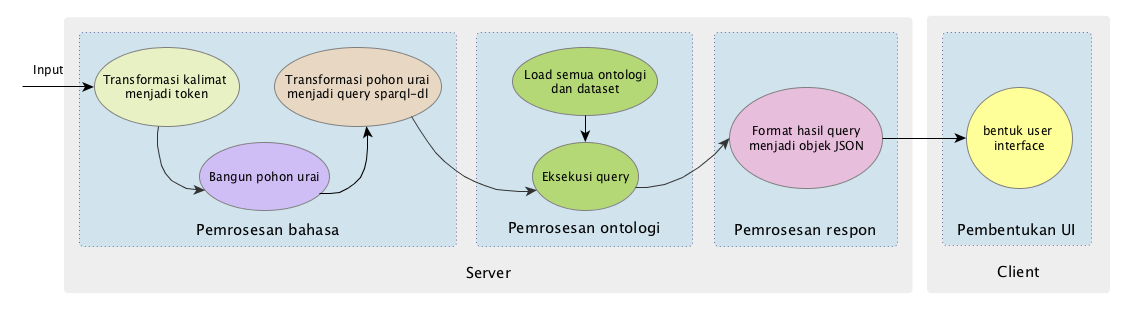
\includegraphics[width=1\textwidth]{bab_4/gambaran_umum_sistem}
	\caption{Gambaran umum sistem}
	\label{fig:gambaran_umum_sistem}
\end{figure}

Proses awal merupakan proses analisa pertanyaan yaitu berkaitan dengan pemrosesan kalimat tanya dimana proses ini merupakan proses transformasi bahasa alami menjadi pohon urai \emph{(parse tree)} sehingga komputer dapat memahami maksud dari pertanyaan yang dimasukkan oleh pengguna. Adapun proses pembentukan \emph{parse tree} diawali dengan melakukan proses POS \emph{(Part Of Speech)} tagging terhadap masing-masing kata penyusun kalimat kemudian tiap kata akan dicek kelas katanya ke dalam basis data \emph{lexicon}. Apabila kelas kata yang bersangkutan tidak ditemukan, maka akan dilanjutkan dengan proses analisa morfologi untuk menentukan kelas kata yang sesuai.

Proses utama terdiri dari proses pemahaman terhadap ontologi dan proses eksekusi \emph{query} berdasarkan pertanyaan yang dimasukkan oleh pengguna. Proses ini dilakukan dengan cara mengubah pohon urai yang sudah dibentuk pada proses awal menjadi \emph{statement query} SPARQL-DL yang kemudian dijalankan oleh \emph{query engine}, hasil proses query kemudian dianalisa untuk menentukan apakah hasil query membutuhkan pencarian informasi tambahan dari DBPedia atau tidak, jika diperlukan untuk mencari informasi tambahan mengenai objek hasil query dan \emph{reasoning}, maka sistem akan melakukan query terhadap \emph{endpoint} SPARQL DBPedia Indonesia. 

Proses akhir adalah proses pembentukan template jawaban yang akan dikirimkan ke sisi \emph{client} dalam format objek JSON \emph{(Javascript Object Notation)} yang selanjutnya di sisi \emph{client} akan ditransformasikan menjadi template HTML untuk ditampilkan pada browser.
